\subsection*{Présentation}
\vspace{1em}
\begin{description}
    \item[Nom - Prénom :]
    \item[Surnom :]
    \item[Âge :]
    \item[Région d'origine :]
    \item[Sexe :]
    \item[Célibataire~?]
    \item[IF, premier choix ou pas ?]
    \item[Des problèmes de santé particuliers ?]
	(pour organiser au mieux la
	    semaine d'inté).
\end{description}

\vspace{1cm}

\subsection*{Photo}
Colle-nous donc une jolie photo de toi. Tout contrevenant s'expose à des
poursuites judIFciaires !

\vspace{3cm}
\orga{images/anonymous.jpg}

\subsection*{Test psychologique}
Élaboré par nos plus grands spécialistes, cette section nous permettra d'en
savoir un peu plus sur toi.

\vspace{1em}

\begin{itemize}

    \item \textbf{Que serais-tu si tu étais...}
    \vspace{-3cm}
    \begin{description}
	\item[Chuck Norris :]
	\vspace{3cm}
	\item[Une série :]
	\vspace{1cm}
	\item[Un droïde :]
	\vspace{1cm}
	\item[Un truc vert :]
	\vspace{1cm}
	\item[Une chanson :]
	\vspace{1cm}
	\item[Un film :]
	\vspace{1cm}
	\item[Une heure de la journée :]
	\vspace{1cm}
    \end{description}
	\vspace{2cm}
	
	\item \textbf{Donne une description précise du rituel  
	 de l'huître et du pingouin :}
    \vspace{7cm}
		
    \item \textbf{Lequel des orgas te paraît le plus sympa ?}
    \newpage
	
    \item \textbf{Un ours des forêts du nord met deux jours pour traverser 500 mètres de forêt. Pourquoi ?}
	\vspace{7cm}
	
    \item \textbf{Que cherches-tu en venant en IF ?}
    \vspace{6cm}
	
    \item \textbf{Dessine-nous un avion à réaction robotisé intelligent avec une
    lueur maléfique dans les yeux et des poils soyeux :}
    \vspace{10cm}
	
    \item \textbf{Pose-nous une question :}
    \vspace{6cm}
	
\end{itemize}

\subsection*{Test de Geekness}
\begin{itemize}

    \item \textbf{Quelle est la différence entre un geek et un nerd ?}
    \vspace{5cm}
	
    \item \textbf{Combien de langages de programmation maîtrises-tu ?}
    \vspace{4cm}
	
    \item \textbf{Explique en 3 points pourquoi les produits Apple ne valent
	pas un clou :}
    \vspace{4cm}

    \newpage

    \item \textbf{Combien d'épisodes de séries regardes-tu chaque
	semaine en moyenne ?} (\emph{parce qu'on est un peu à cours, dans l'équipe})
    \vspace{3cm}
    
    \item \textbf{Tu utilises plutôt quotidiennement :}
    \begin{description}
	\item[$\square$] Microsoft Windows.
	\item[$\square$] GNU/Linux.
	\item[$\square$] Apple -- Mac OS.
	\item[$\square$] BSD -- Solaris -- un Atari -- un Amiga.
	\item[$\square$] Un verre à pintes.
	\item[$\square$] Mais qu'est-ce que je fais là ?!
    \end{description}
	\vspace{2em}
	
    \item \textbf{L'info, pour toi, c'est :}
    \begin{description}
	\item[$\square$] Une passion.
	\item[$\square$] Un moyen de se faire pas mal d'argent.
	\item[$\square$] Un bon moyen de faire du management plus tard.
	\item[$\square$] Ta vie.
	\item[$\square$] Un outil.
	\item[$\square$] Marrant.
	\item[$\square$] 42.
    \end{description}
	\vspace{2em}
	
    \item \textbf{T'as deux heures à tuer, tu fais quoi ?}
    \begin{description}
	\item[$\square$] T'as justement une classe à écrire sur un de tes projets.
	\item[$\square$] Tu prends un bon bouquin.
	\item[$\square$] T'appelles un pote et tu vas prendre un café en ville.
	\item[$\square$] Tu joues à un jeu (vidéo, ou pas).
	\item[$\square$] Tu fais du sport.
	\item[$\square$] Tu crées un truc (dessin, musique, cuisine, UML, etc.).
    \end{description}
	\vspace{2em}
	
    \item \textbf{Comment appelle-t-on ceci ?}
    \begin{verbatim}
	#include<stdio.h>
	char*f="char*f=%c%s%c;main()"
	"{printf(f,34,f,34,10);}%c";
	main(){printf(f,34,f,34,10);}
    \end{verbatim}
    \vspace{8cm}
	
    \item \textbf{Une passion dévorante ?} (sport, musique, dessin, etc.)
    \vspace{4cm}
	
    \item \textbf{Des projets notables en info ?} (i.e. utilisés par plus de monde que ta grand-mère, toi, et le prof qui t'a corrigé...)
    \vspace{4cm}

\end{itemize}

\subsection*{Encore une photo}
Colle ici une photo de toi complètement stupide :
\begin{center}

\includegraphics[height=5cm, angle=120]{images/anonymous.jpg}
\end{center}
Les meilleures photos gagneront un passage sur
\url{http://bonjourlesifs.tumblr.com}.


\subsection*{Presque la fin...}
Marque-nous quelque chose. Oui, n'importe quoi. Non, vraiment, tu peux te
lâcher, vas-y. Y a même de la place pour dessiner, écrire de la musique, alors soit inventif, cet
espace est rien que pour toi !

\vfill

\columnbreak

\subsection{Mais qu'est-ce que je fais avec toutes ces questions ?}
C'est pas bien compliqué, tu les renvoies avec le coupon réponse pour le WEI et
ton chèque de 25 euros à :
\vspace{1em}
\adresseCoupon
\vspace{1em}


Fais quand même attention, le chèque pour le WEI est à mettre à l'ordre de \textbf{AEDI}, pas de la personne ci-dessus !

\vfill
\hspace{-5cm}
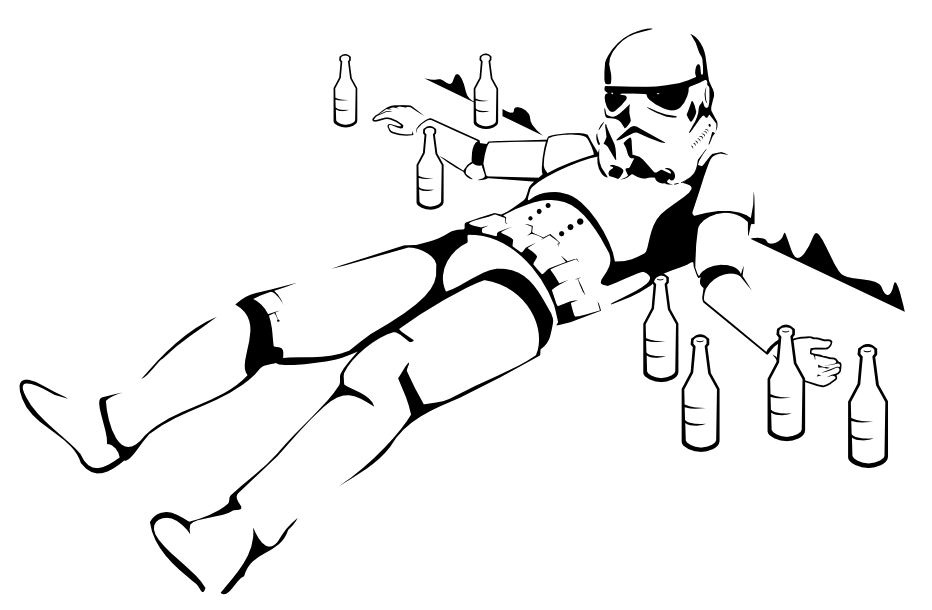
\includegraphics[height=8cm]{images/stormTrooperBourre.png}
